%% The following is a directive for TeXShop to indicate the main file
%%!TEX root = diss.tex

\chapter{Cross-modal word identification}
\label{chap:sent}

%This chapter investigates perceptual learning with a different bias than lexical, by using sentential context to bias participants towards a particular word.

\section{Motivation}

In Chapter~\ref{chap:lexdec}, listeners showed greater perceptual learning effects when the lexical bias was greater.  
However, this relationship was not found when attention was drawn to the ambiguous sound and when the ambiguous sound was farther from the canonical production.  
The experiment in this chapter seeks to increase the linguistic expectations for the words containing the ambiguous productions as a way to induce more comprehension-oriented attentional sets, even in the face of explicit instructions promoting perception-oriented attentional sets.  
To this end, semantic predictability is used to boost linguistic expectations in conjunction with lexical bias.

Semantic predictability in production studies has been found to have an effect on vowel realization and duration independent of lexical factors such as frequency and neighbourhood density \citep{Scarborough2010, Clopper2008}.  
In speech perception work, semantic predictability has been found to have an effect on phoneme categorization similar to that of lexical bias \citep{Borsky1998}, and increased intelligibility in noise, particularly for native speakers \citep[and others]{Kalikow1977, Mayo1997, Fallon2002, Bradlow2007}.
In phoneme restoration, semantic predictability both increased the bias to respond that a word intact and also increased the sensitivity to noise addition versus noise replacement \citep{Samuel1981}.

As in previous work, two levels of semantic predictability are used in this experiment.  
Highly predictable sentences are ones where the final word is constrained to only a few words.  
Unpredictable sentences are ones where the possible completions are numerous, and any completions given are more guesses than anything else.
All target words and the threshold for ambiguity are taken from Experiment 1 and have the highest lexical bias available.
When a listener is exposed to these words in unpredictable sentences, they should show perceptual learning effects equivalent to those participants in the S-Final condition of Experiment 1.

The exposure task in this experiment differs from lexical decision task used in the previous chapter.  
Instead, participants identify the picture that matches the final word in the sentence, and all trials involve a real word.
The attentional set for this task, where participants make a decision about the identity of a specific word, may be different from the previous experiment, where they make a decision about the lexicality of a word, but the decision is about the word in both instances.

If linguistic expectations are cumulative, we should expect to see a larger perceptual learning effect for participants exposed to ambiguous sounds in words that are highly predictable, due to greater use of comprehension-oriented attentional sets.
Additionally, if the explicit attention does exert a categorical effect on perceptual learning, we should see a similar size of perceptual learning in this experiment in the attention conditions as in the previous experiments.
Previous research has found an increased sensitivity to signal properties in semantically predictable sentences \citep{Samuel1981}, which could lead to one of two outcomes.
Given that bias to restore the phoneme was greater in these conditions as well, we might see greater perceptual learning effects, as the link between the word and the production would be enhanced, but the signal would be encoded more accurately from the lower cognitive load.
On the other hand, the lower cognitive load could lead to more attention available to notice the deviant production, and thus adopt a perception-oriented attentional set.
Also relevant are the findings of \citet{Kraljic2008a}, where no perceptual learning was observed when the modified sound was in a /str/ context.
In that context, the modified sound was not salient, and no learning was observed.
If participants do not pay attention to the final word in a predictable sentence, perceptual learning might also be reduced or absent.

\section{Methodology}

\subsection{Participants}

One hundred native speakers of English participated in the experiment and were compensated with either \$10 CAD or course credit. 
They were recruited from the UBC student population.  
Twenty additional native English speakers participated in a pretest to determine sentence predictability, and 10 other native English speakers participated in a picture naming pretest.
Participants were native North American English speakers with no reported speech or hearing disorders.

\subsection{Materials}

One hundred and twenty sentences were used as exposure materials.  
The set of sentences consisted of 40 critical sentences, 20 control sentences and 60 filler sentences. 
The critical sentences ended in one of 20 of the critical words in Experiments 1 and 2 that had an /s/ in the onset of the final syllable.  
The 20 control sentences ended in the 20 control items used in Experiments 1 and 2, and the 60 filler sentences ended in the 60 filler words in Experiments 1 and 2.  
Half of all sentences were written to be predictive of the final word, and the other half were written to be unpredictive of the final word.  
Unlike previous studies using sentence or semantic predictability \citep{Kalikow1977}, Unpredictive sentences were written with the final word in mind with a variety of sentence structures, and the final words were plausible objects of lexical verbs and prepositions.  
A full list of words and their contexts can be found in the appendix. Aside from the sibilants in the critical and control words, the sentences contained no sibilants (/s z \textesh\ \textyogh\ \textteshlig\  \textdyoghlig/).  
The same minimal pairs for phonetic categorization as in Experiments 1 and 2 were used.

Sentences were recorded by the same male Vancouver English speaker used in Experiments 1 and 2.  
Critical sentences were recorded in pairs, with one normal production and then a production of the same sentence with the /s/ in the final word replaced with an /\textesh/.  
The speaker was instructed to produce both sentences with comparable speech rate, speech style and prosody.

As in Experiments 1 and 2, the critical items were morphed together into an 11-step continuum using STRAIGHT \citep{Kawahara2008}; however, only the final word in sentence was morphed.  
For all steps, the preceding words in the sentence were kept as the natural production to minimize artifacts of the morphing algorithm.  
The control and filler items were also processed and resynthesized to ensure consistent quality.  The ambiguous point selection was based on the pretest performed for Experiment 1 and 2 exposure items.  
The ambiguous steps of the continua chosen corresponded to the 50\% cross over point in Experiment 2.

Pictures of 200 words, with 100 pictures for the final word of the sentences and 100 for distractors, were selected in two steps.  
First, a research assistant selected five images from a Google image search of the word, and then a single image representing that word was selected from amongst the five by me.  
To ensure consistent behaviour in E-Prime, pictures were resized to fit within a 400x400 area with a resolution of 72x72 DPI and converted to bitmap format.  
Additionally, any transparent backgrounds in the pictures were converted to plain white backgrounds.

\subsection{Pretest}

The same twenty participants that completed the lexical decision continua pre-test also completed a sentence predictability task before the phonetic categorization task described in Experiment 1. 
Participants were compensated with \$10 CAD for both tasks, and were native North American English speakers with no reported speech, language or hearing disorders. In this task, participants were presented with sentence fragments that were lacking in the final word.  
They were instructed to type in the word that came to mind when reading the fragment, and to enter any additional words that came to mind that would also complete the sentence.  
There was no time limit for entry and participants were shown an example with the fragment ``The boat sailed across the...'' and the possible completions ``bay, ocean, lake, river''.  
Responses were collected in E-Prime (cite), and were sanitized by removing miscellaneous keystrokes recorded by E-Prime, spell checking, and standardizing variant spellings and plural forms.

The measure used for determining rewriting of sentences was the proportion of participants that included the target word in their responses.  
For predictive sentences, the mean proportion was 0.49 (range 0-0.95) and for unpredictive sentences, the mean proportion was 0.03 (range 0-0.45).  
Predictive sentences that had target response proportions of 20\% or less were rewritten.  
The predictive sentences for \emph{auction}, \emph{brochure}, \emph{carousel}, \emph{cashier}, \emph{cockpit}, \emph{concert}, \emph{cowboy}, \emph{currency}, \emph{cursor}, \emph{cushion}, \emph{dryer}, \emph{graffiti}, and \emph{missile} were rewritten to remove any ambiguities.  

Five volunteers from the Speech in Context lab participated in another pretest to determine how suitable the pictures were at representing their associated word.  
All participants were native speakers of North American English, with reported corrected-to-normal vision. Participants were presented with a single image in the middle of the screen.  
Their task was to type the word that first came to mind, and any other words that described the picture equally well.  
There was no time limit and presentation of the pictures was self-paced. Responses were sanitized as in the first pretest.  

Pictures were replaced if 20\% or less of the participants (1 of 5) responded with the target word and the responses were semantically unrelated to the target word. 
Five pictures were replaced, \emph{toothpick} and \emph{falafel} with clearer pictures and \emph{ukulele}, \emph{earmuff} and \emph{earplug} were replaced with \emph{rollerblader}, \emph{anchor} and \emph{bedroom}.  
All five replacements were for distractor words.

\subsection{Procedure}

As in Experiments 1 and 2, participants completed two tasks, an exposure task and a categorization task.  For the exposure task, participants heard a sentence via headphones for each trial.  Immediately following the auditory presentation, they were presented with two pictures on the screen.  Their task was to select the picture on the screen that corresponded to the final word in the sentence they heard.  As in Experiments 1 and 2, the order was pseudorandom, with the same constraints.

Participants were assigned to one of four groups of 25 participants.  
In the exposure phase, half of the participants were exposed to a modified /s/ sound only in Predictive sentences and half were exposed to it only in Unpredictive sentences.  
Half of all participants were told that the speaker's production of ``s'' was sometimes ambiguous, and to listen carefully to ensure correct responses.  

Following the exposure task, participants completed the same categorization task described in Experiments 1 and 2.

\section{Results}

\subsection{Exposure}

Performance in the task was high, with accuracy near perfect across all subjects (mean accuracy = 99.5\%, sd = 0.8\%).  A linear mixed effects model for logarithmically-transformed reaction time revealed no significant differences as a result of condition.

\subsection{Categorization}

Responses with reaction times less than 200 ms or greater than 2500 ms were excluded from analyses. 
A logistic mixed effects model was constructed with Subject and Continua as random effects and continua Step as random slopes, with 0 coded as a /\textesh/ response and 1 as a /s/ response.  Fixed effects for the model were Step, Exposure Type, Attention and their interactions, with deviance coding used for contrasts for Exposure Type (Unpredictive = 0.5, Predictive = -0.5) and Attention (No attention = 0.5, Attention = -0.5).


\begin{figure*}[!ht]
\caption{Proportion /s/ response along the 6 step continua as a function of Exposure Type and Attention in Experiment 3.  Error bars represent 95\% confidence intervals.}
\label{fig:exp3categ}
\begin{center}
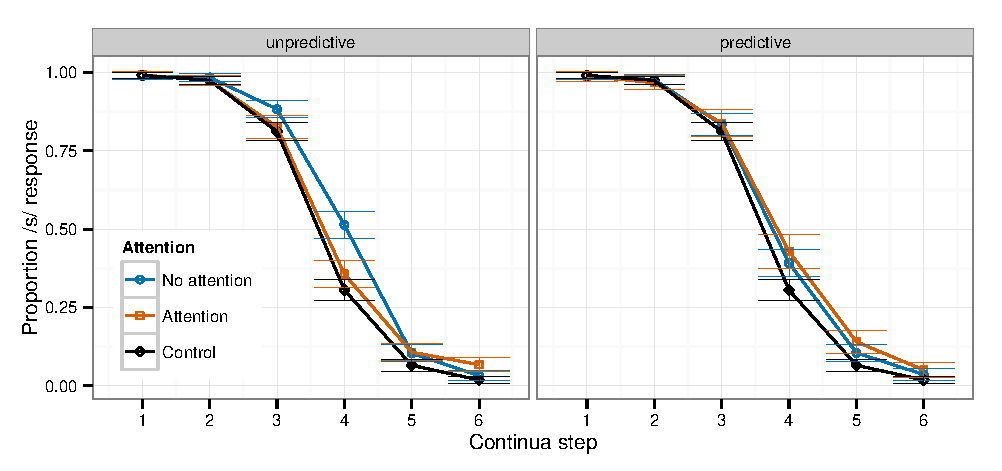
\includegraphics[width=\textwidth]{graphs/exp3_categresults}
\end{center}
\end{figure*}

As in the previous experiments, there was a significant effect of the intercept ($\beta = 0.52, SE = 0.20, z = 2.6, p < 0.01$) and of Step ($\beta = -2.49, SE = 0.19, z = -12.7, p < 0.01$).
Exposure Type ($\beta = 0.23, SE = 0.23, z = 0.97, p = 0.33$), Attention ($\beta = 0.30, SE = 0.21, z = 1.4, p = 0.15$), and their interaction ($\beta = 0.38, SE = 0.44, z = 0.9, p = 0.39$) are all not significant, despite the visible differences in Figure~\ref{fig:exp23categ}.


\begin{figure*}[!ht]
\caption{Proportion /s/ response along the 6 step continua as a function of Exposure Type and Attention in Experiment 3 and the word-medial condition of Experiment 1.  Error bars represent 95\% confidence intervals.}
\label{fig:exp23categ}
\begin{center}
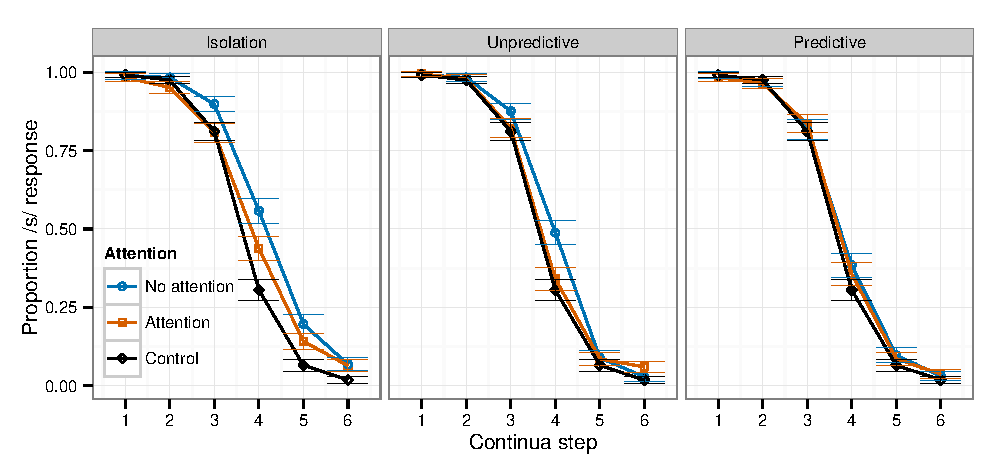
\includegraphics[width=\textwidth]{graphs/exp23_categresults}
\end{center}
\end{figure*}


As an additional comparison, the data from this experiment was combined with the subset of participants in Experiment 1 who were exposed to the same set of words (the word-medial condition).  
Exposure Type was recoded as a three-level factor, using treatment (dummy) contrast cpdomg, with the Experiment 1 exposure (Isolation) as the reference level. 
An identically specified logisitic mixed effects model was fit to this set data as to the initial data.  
In this model, there was a significant effect of Attention ($\beta = 0.74, SE = 0.32, z = 2.2, p = 0.02$), such that participants in Attention conditions were less likely to categorize the continua steps as /s/.  
Additionally, Exposure Type had a marginal effect of Predictive compared to Isolation ($\beta = -0.43, SE = 0.23, z = -1.9, p = 0.05$) and two significant interactions, one between Step and Unpredictive ($\beta = -0.42, SE = 0.17, z = -2.4, p = 0.01$) and one between Step and Predictive ($\beta = -0.32, SE = 0.14, z = -2.2, p = 0.02$).  
These marginal effect of Predictive indicates that participants in that condition were less likely categorize the continua as /s/ overall, and the interactions between the sentential conditions and Step indicate that the slope of categorization functions, as seen in Figure~\ref{fig:exp23categ}, were significantly steeper than in the Isolation condition.
Attention and Exposure Type did not significantly interact.

Two additional models were run with the reference level for Exposure Type as Predictive and Unpredictive.  In the model with Predictive as reference, the intercept is no longer significant ($\beta = 0.44, SE = 0.28, z = 1.5, p = 0.12$), indicating percpetual learning was not robustly present in participants in the Predictive condition.  The difference between the Predictive condition and the Isolation condition remains ($\beta = 0.77, SE = 0.32, z = 2.4, p = 0.01$), and, as above, the difference between Predictive and Unpredictive is not significant ($\beta = 0.42, SE = 0.31, z = 1.3, p = 0.17$). ##Doublecheck these numbers, degenerate hessian for one


\section{Discussion}

One key finding of the current experiment is that modified categories embedded in words in meaningful sentences produce less perceptual learning than words in isolation.  Particularly, as the predictability of the context increases, the amount of perceptual learning decreases.  In fact, participants exposed to a modified category only in predictive words did not have a significantly different category boundary than the middle of the continua. 

Figure~\ref{fig:exp13xoverdist} shows the distributions of cross over points across the word-final conditions of Experiment 1 (labeled as Isolation) and all conditions of Experiment 3, with the distribution of the control experiment for comparison.  Across all exposure types, there is a clear tendency for speakers in the Attention conditions to have smaller perceptual learning effects than their No attention counterparts.  The distribution of the crossover points of participants from Experiment 1 have a larger standard deviation than those involving sentential contexts, but outliers are most prevalent in the Predictive condition with No attention.  This abundance of outliers is likely due to a relative lack of constraint on the attentional set required by the task.  In all other conditions, participants are guided toward perception-oriented attentional sets, either through a lack of contextual cues or through explicit attention.

\begin{figure*}[!ht]
\caption{Distribution of cross over points for each participant across comparable exposure tokens in Experiments 1 and 3.}
\label{fig:exp13xoverdist}
\begin{center}
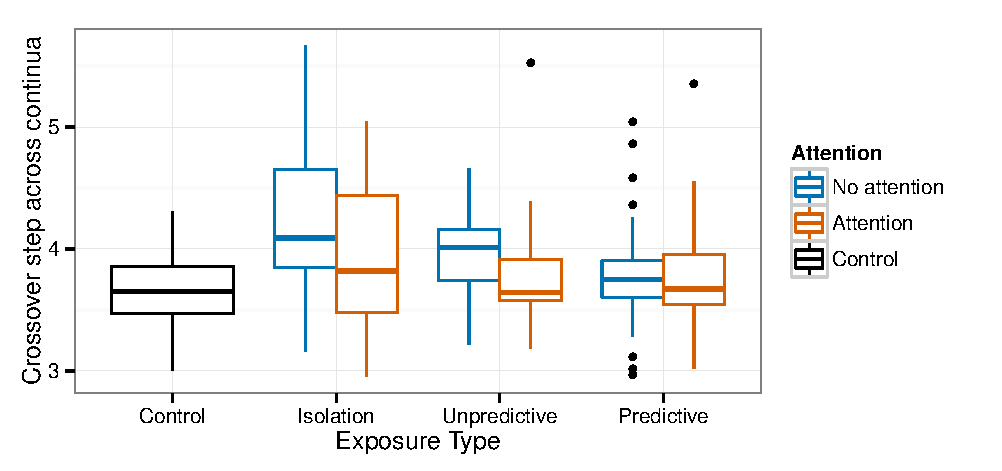
\includegraphics[width=\textwidth]{graphs/exp13_xoverdist}
\end{center}
\end{figure*}

There are several potential explanations for the lack of perceptual learning observed in the participants who heard the modified sound category only in predictable sentences.
The first is that when the sentence is predictive of the final word, participants simply did not use the actual production of the final word for their resposne.  
That is, because the task was to identify the correct picture as fast as possible, the available information earlier in the sentence provided sufficient information to render a decision, so processing the final word was not necessary.  An experiment that would shed light on whether this explanation is valid would be one that looked at differences in form encoding.  For instance, if the form encoding is impoverished, long-term form priming would be affected, but long-term semantic priming would not be.  For unpredictive sentences, both long-term form priming and semantic priming should be to be as robust as such priming for words in isolation.

Another potential explanation for the lack of perceptual learning effects observed is that predictive sentences are lower cognitive load than unpredictive sentences, as put forth by \citet{Samuel1981}, where it wa found that listeners are more sensitive to signal properties of words in predictive contexts.  In line with that reasoning, the reduced cognitive load in predictive sentences would allow listeners to attend to the signal more easily, reducing the perceptual learning, as in the previous two experiments.  However, perceptual learning effects were still observed in those experiments, whereas it appears to be absent entirely for the participants exposed to the sound category in predictive sentences.
